\chapter{Coverage path planning problem} 


\minitoc

The following section is dedicated to the Coverage Path Planning (named CPP). Until now the work presented was focus on optimizing the position and orientation of a fix number of cameras to cover an vast and complex area. 
The method introduced using GA or a more flexible (but slower) GAPSO, give an efficient result to estimate the pose of a set of fix cameras. Instead to place several cameras at each poses estimate, the poses are considered as waypoints. 
The detail of the proposed solution to optimize the CPP problem and few experiments made are presented in these sections.
 

\section{Sequential method}
To optimize the CPP problems a simple and innovative method has been developed. The method proposed here can be decomposed in 3 principal part all interconnected. 
\begin{itemize}
	\item Number of waypoints : 
	A crucial step is to estimate the number of waypoints. A wrong estimation with a too high or to low will cause au  bad area coverage or the next computation to complex.
	\item Waypoints positioning : 
	The waypoints positioning optimization is the more crucial step. As already discuses numerous solution has been studied to optimize the pose of the cameras depending several constraint. Based on it and the experiment made until now, an efficient algorithms has been chosen and adapted to pose estimate each waypoint (see \ref{sec:hybridGAPSO}). 
	\item  Path plan computation : 
	 When the number and the position of the waypoints has been computed the last step is to find the shorter route  passing by all the waypoints with must start and finish at the same position (as the TSP \ref{sec:TSP}).
	
	% the number of waypoints will cause a  more complex and longer estimation of the pose for each of them and increase the complexity to compute a path. Otherwise with a too low number of waypoint the area will not be well cover and leave some black hole. 
\end{itemize}

The method propose has the advantage to optimize independently all the waypoints and the path plan. This method is also not systematically based on a sweep and allows to have shorter path with the same stating point and ending point. 


\subsection{Number of waypoint and their poses estimation}\label{sec:NmbWaypoint}

Is difficult to estimate properly the minimum of waypoints which are necessary to cover a complex area.
To do so, a two-step procedure has been implemented. Based on the pose optimization of a fixed number of waypoints introduce in the precedent Chapter \ref{chap:waypointPoseExp}. 
The first step is to find the minimum number of waypoints depending on the area to cover like formulated in the
 Equation \ref{Eq:waypointN}. \\
\begin{equation}\label{Eq:waypointN}
\frac{ A_{room} - \sum_{i=1}^n A_{wall i} }{A_{cam}} \times \mbox{Threshold Rate} = \mbox{NWayPoint}
\end{equation}

\begin{itemize}
\item[-] $ A_{room}: $  area of the Room (length $\times$ width)
\item[-] $ A_{Wall}: $  area of the obstacle like wall (length $\times$ width)
\item[-] $ A_{Cam}: $   area cover by the camera in the maximum size of $z$
\item[-] $ \mbox{NWayPoint}: $  number of waypoints
\item[-] $ \mbox{Threshold Rate}: $ objective threshold rate 
\item[-] $S:$ one solution of waypoints set 
\item[-] $evalCost:$ cost function  
\end{itemize}

The second step is to compute GA optimization until the threshold is reached. At the end of each GA convergence if the threshold rate is not reached one more waypoints is added and the GA optimization restart with one more waypoints. The algorithm  used to estimate the number of waypoint  is explained in the "Algorithm 1 Estimation of the number of waypoints".  
               %  while increasing the number of waypoints like explained in the Algorithm 1 Estimation of the number of waypoints.  

\begin{algorithm}{}
\caption{Estimation of the number of waypoints}\label{alg:euclid}
\begin{algorithmic}[6]
\Procedure{NmbWaypoint}{$A_{room},A_{Wall},\mbox{Threshold Rate},A_{Cam}$}
 \State $S\gets 0$
  \State $NWayPoint\gets \frac{ A_{room} - \sum_{i=1}^n A_{wall i} }{A_{cam}} \times \mbox{Threshold Rate} 
 $  (Equation \ref{Eq:waypointN})
  \While{$eval Cost(S)\leq ThresholdRate$}
	 \State $S \gets GA(NWayPoint)$
	  \State $NWayPoint\gets NWayPoint+1$
  \EndWhile\label{endwhile}
\State \textbf{return} $NWayPoint$
\EndProcedure
\end{algorithmic}
\end{algorithm}

At the end of these steps, we have the number and a good set of waypoints pose from the last GA convergence. The waypoints pose can directly be used, but can also be refined using the adapted PSO (as in the GAPSO see \ref{sec:hybridGAPSO}). Once the number and the efficient pose of the waypoints done the next step is to compute the path planning.  
%%%%%%%%%%%%%%%%%%%%%%%%%%%%%%%%%%%%%%%%%%%%%%%%%%%%%%%%%%%%%%%
%%%%%%%%%%%%%%%%%%%%%%%%%%%%%%%%%%%%%%%%%%%%%%%%%%%%%%%%%%%%%%%%%%%%%%%%%%%%%%%%%%%%%%%%%%%%%%%%%%%%%%%%%%%%	
	
% \begin{mfigures}[!]{optimisation of the path plannig}{fig:Path_planning} \centering
%\mfigure{width=.4\linewidth}{img/22pts_WaypointsDijktra2.jpg}{Poses of every image captured in the room.}{subfig:Dijktra}
%\hspace{1cm}
%\mfigure{width=.4\linewidth}{img/22pts_WaypointsGA2.jpg}{Path compute with Dijktra multi goal.}{subfig:GATSP}
%\end{mfigures} 
 
  \subsection{Sorted waypoints and path planning.} \label{sorted}
In the previous section, the method to obtain the small list of waypoints to have a desired coverage has been detailed. The list of waypoints has to be sort to compute an efficient path with shorter travelling distance. In order to create an efficient path passing by all optimised waypoints the problem is formalized as a TSP. The TSP  quickly described in the flowing section.

% \subsubsection*{a)}{Shortest Path Problem}
% \\Normally, finding a shortest path between two points in configuration space is mature enough. In our case we assume the waypoints as multi goals. So the planning in this method will simply find at every waypoint the shortest Euclidean distance from the other available non-traversed waypoints. Based on that a ranked waypoints list will be generated. This will not guarantee a globally shortest distance, but will only choose the shortest distance every time a waypoint is visited.
 
\subsubsection*{Traveling Salesman Problem. }\label{sec:TSP2}

%%%%%%%%%%%%%%%%%%%%
% \begin{figure}[htp]
%   \centering
%   \subfloat[Image d'origine]{\label{fig:edge-a}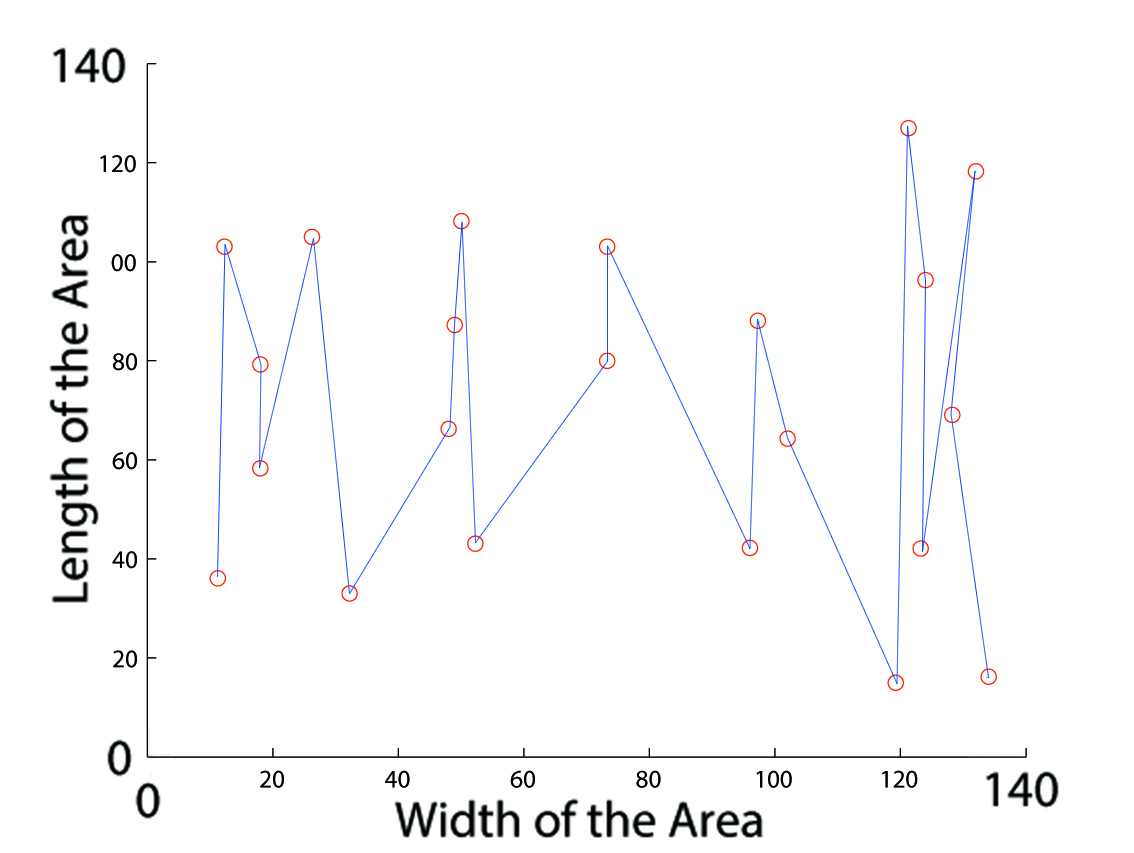
\includegraphics[scale=0.75]{22pts_WaypointsDijktra2.jpg}}
%   \hspace{5pt}
%   \subfloat[Après une détection des contours de Laplace]{\label{fig:contour-b}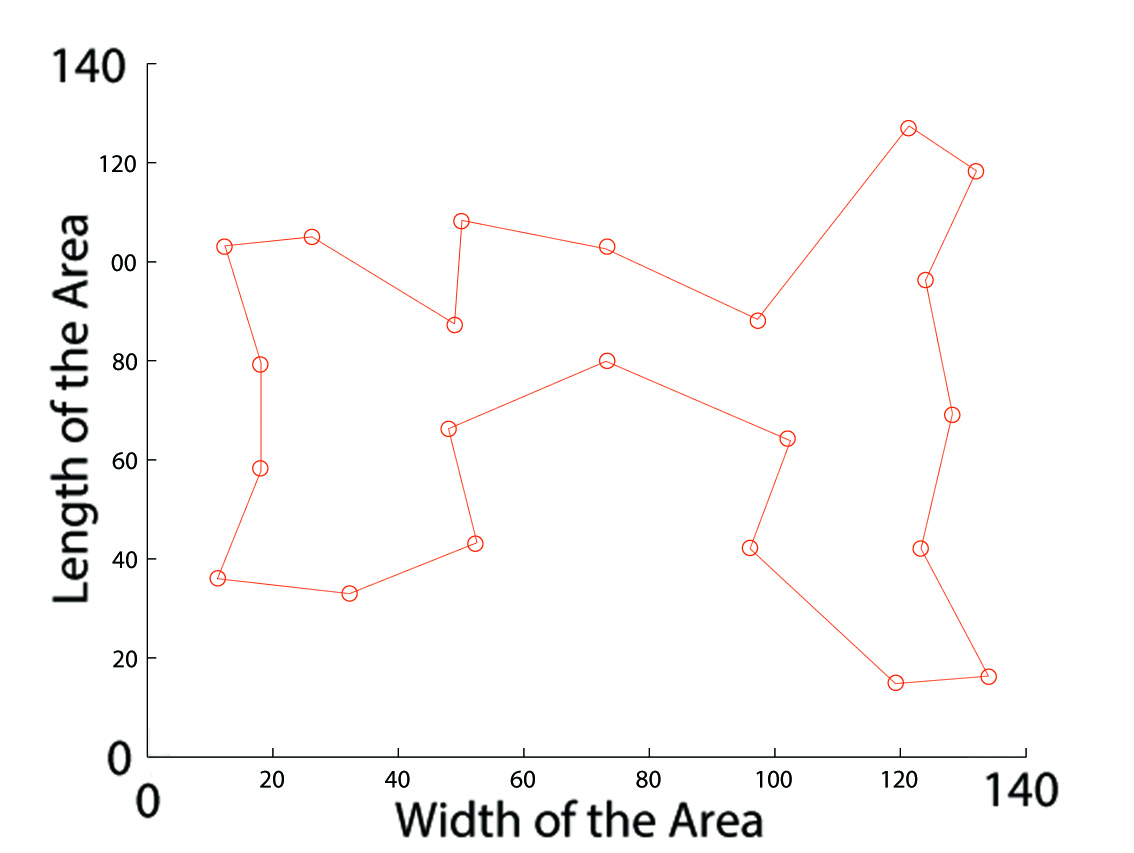
\includegraphics[scale=0.75]{22pts_WaypointsGA2.jpg}}
%   \label{fig:contour}
% \end{figure}
%%%%%%%%%%%%%%%%%%%%

\begin{mfigures}[!]{Optimization of the path planning.}{fig:Path_planning} \centering
\mfigure{width=.4\linewidth}{img/fig5-a.png}{Every pose after the optimization of the waypoint positioning. }{subfig:Path_planning1}
\hspace{1cm}
\mfigure{width=.4\linewidth}{img/fig5-b.jpg}{Path compute with GA multi objective for TSP.}{subfig:Path_planning2}
\end{mfigures}	

The sorted path can be formulated as travelling salesman problem (TSP). To remember the travelling salesman problem (TSP) is inspired by a question asked by a salesman  "\textbf{What is the shortest path passing by each city only one time and return to the starting city? When i know a list of cities and the distances between each pair of cities. }". The TSP problem is a well known NP-Hard and NP-complete problem ( see \citep{236*karp1972}) and different solutions exit to optimize it depending of the context. 
Ponnambalam et al 172* \cite{172*} propose to use the GA adapted to  multi-objective to optimize the TSP, also provide the GA set-up(mutation rate, population size...). DAVIES et al \cite{56*davies2006} propose also to use the GA to solve the TSP applied on robotic with an obstacle constraint. \\
Based on the literature, the GA since adapted and efficient enough to optimize the TSP problems.
The GA  has to be set-up properly depending then the problem specific to TSP. The GA set-up was discussed in the section \ref{sec:Setting and set-up}. About the set-up the more appropriate to optimize the TSP, several studies has been made  as  \citep{68*muhlenbein1989,80*serpell2010,139*razali2011}139*. The conclusion is to use an simple GA for combinator problem. That mean the operator has to be adapted (using swap for example) with an high mutation rate and a very elitist selection.
One example  using a adapted GA solution is provided in the Figure \figref{fig:Path_planning}



%\texttt{\begin{figure}[t!]
%  \centering
%   \subfloat[ Every pose after the optimization of the waypoint positioning.  ]{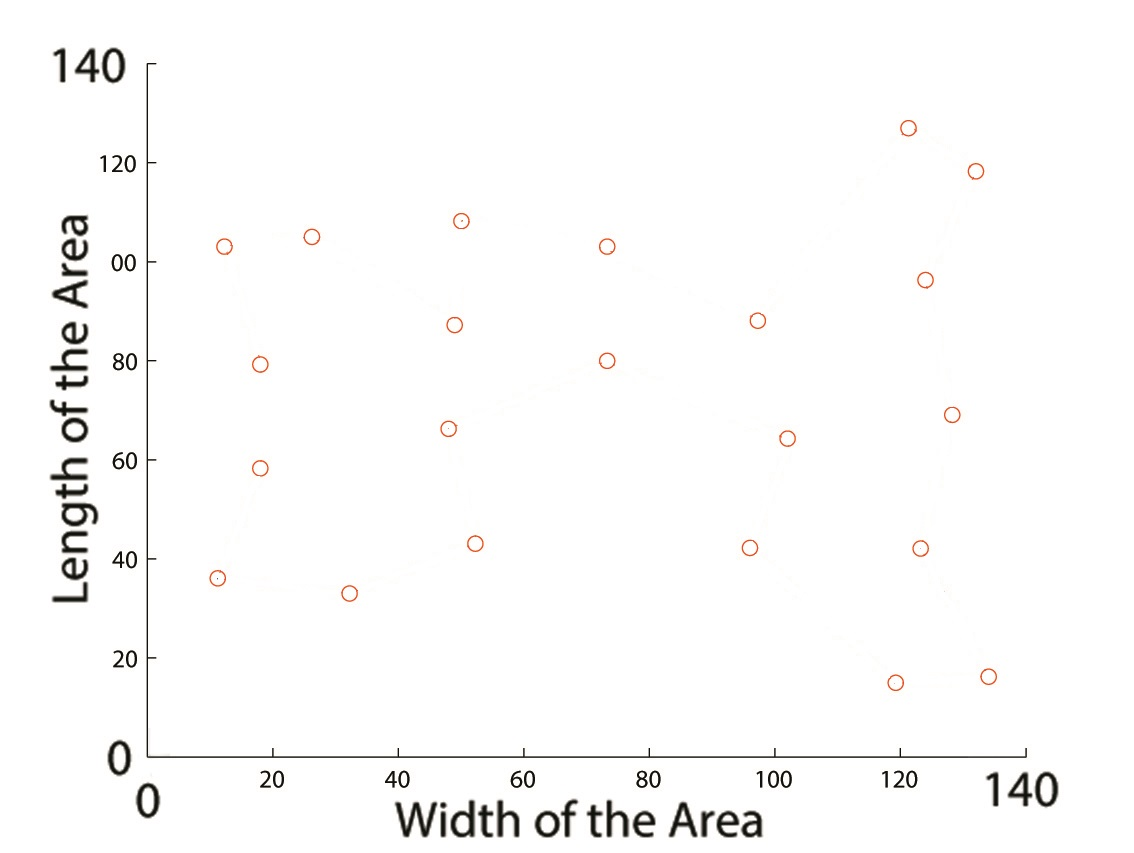
\includegraphics[width=0.45\textwidth]{fig5-a.png}}
%   \hfill
%   \subfloat[Path compute with GA multi objective for TSP. ]{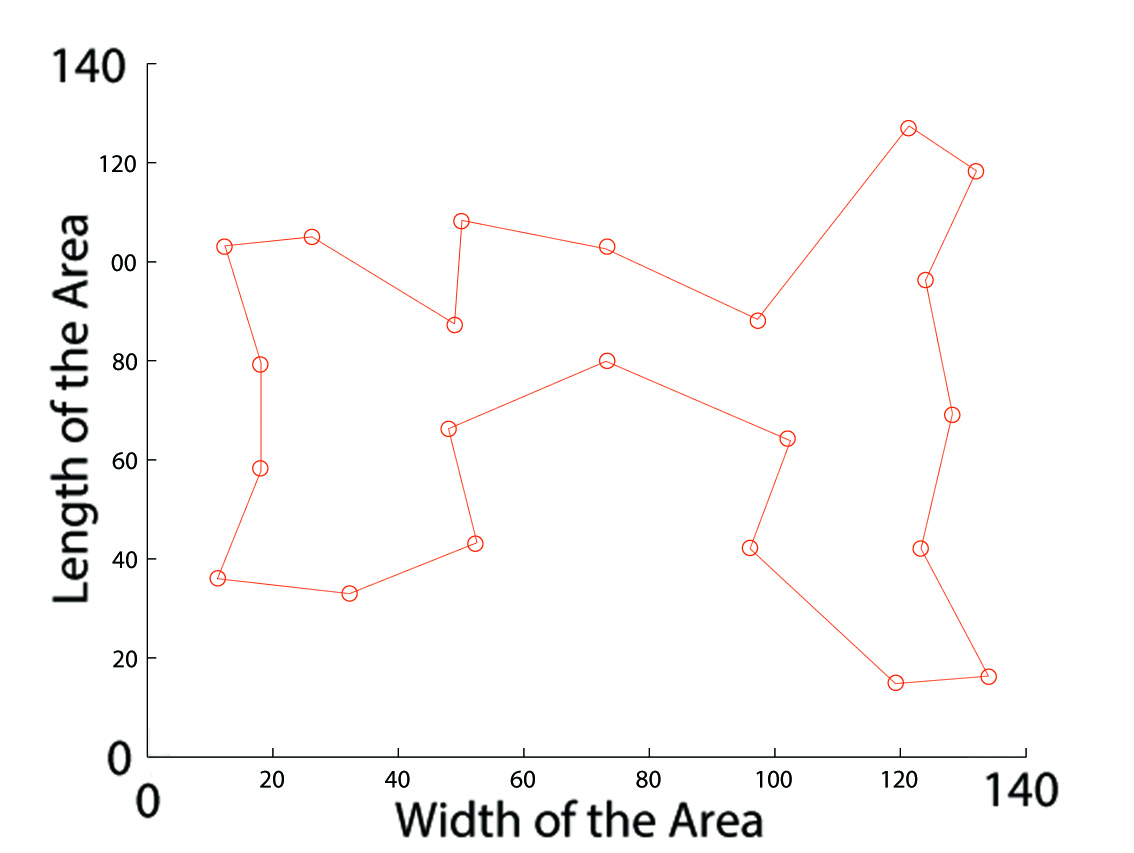
\includegraphics[width=0.45\textwidth]{fig5-b.jpg}}
%  \caption{Optimization of the path planning.}\label{fig:Path_planning} 
%\end{figure}}
% Every node which is a point in space is represented as a city and the Euclidean distances between the cities are calculated and used as a cost function. The path is organized based on the minimum distance traversing over all the cities (or waypoints). To find an optimized solution GA is here again used.

% The privilege of TSP problem formulation and solving it using GA over the other shortest path algorithms like Dijkstra, is that it provides global  complete solution traversing all the waypoints not finding a path from a starting node  to a goal node. The GA approach is more clarified and discussed by Trevor \textit{et al}     \cite{GA_Path}. 
%  The distance covered by a path that is planned by GA is 513 meters, which is shorter by the factor of 1.8 compared to the distance covered by Dijsktra multi goal approach which is 963 meters. Using the GA  to optimize  the scheduling problem of waypoint makes a more efficient result and especially the GA unlike the Dijsktra multi goal, it is more efficient to sort a high number of waypoints.\\ 
 
\subsubsection{Complexity of trajectory. }\label{tarjectory}

Once the waypoints position estimated and the shorter path passing by all the waypoints computed it is interesting to can evaluate the trajectory complexity. The trajectory complexity can be a good glue of the path reliability.  
 
To estimate the trajectory, two indicators are used in order to evaluate properly the path complexity. The first indicator is the distance of the trajectory. The distance allow to evaluate basically the optimization of the path planning. This indicator is directly include in the optimisation process as discussed before \ref{sec:TSP2}. 
Evaluate the trajectory only by using the distance indicator is not enough and an other indicator must be associate to can evaluate quickly the trajectory complexity. To estimate the complexity in terms of curve for the UAV evolving in the 3D space the several angles at each node is studied. 
The complexity of trajectory indicator is computed as follow: 
\begin{equation}\label{Eq:trajectory}
\mbox{Trajectory complexity}=\frac{ \sum_{i=1}^{size(\alpha)} 180- \alpha_{i}  }{size(\alpha)}   
\end{equation}
Where $\alpha_i$ is an angle of curve in the trajectory as in Figure \figref{fig:trajectoirAlpha}. \\
$Size(\alpha)$ is the number of curve in all the trajectory.\\ 
This method  can give an idea of the global trajectory complexity despite this simplicity. 
The two indicator presented (the distance and the trajectory complexity) are used during the next section  to evaluate the gain of the proposed method.
	
 \begin{mfigures}[!]{optimisation of the path plannig}{fig:trajectoirAlpha} \centering
\mfigure{width=.4\linewidth}{img/TrajectoirAlpha3.png}{Extraction of the curve angle in the trajectory.}{subfig:trajectoirAlpha}
\end{mfigures} 
%%%%%%%%%%%%%%%%%%%%%%%%%%%%%%%%%%%%%%%%%%%%%%%%%%%%%%%%%%%%%%%%%%%%%%%%%%%%%%%%%%%%%%%%%%%%%%%%%%%%%%%%%%%%%
	
	
				



%%%%%%%%%%%%%%%%%%%
			\section{Experiment}
		\subsection{Comparison of the trajectory} \label{trajectoire path}
 
% \begin{figure}[t]
%  \centering
%   \subfigure[Path planing using the pattern method]{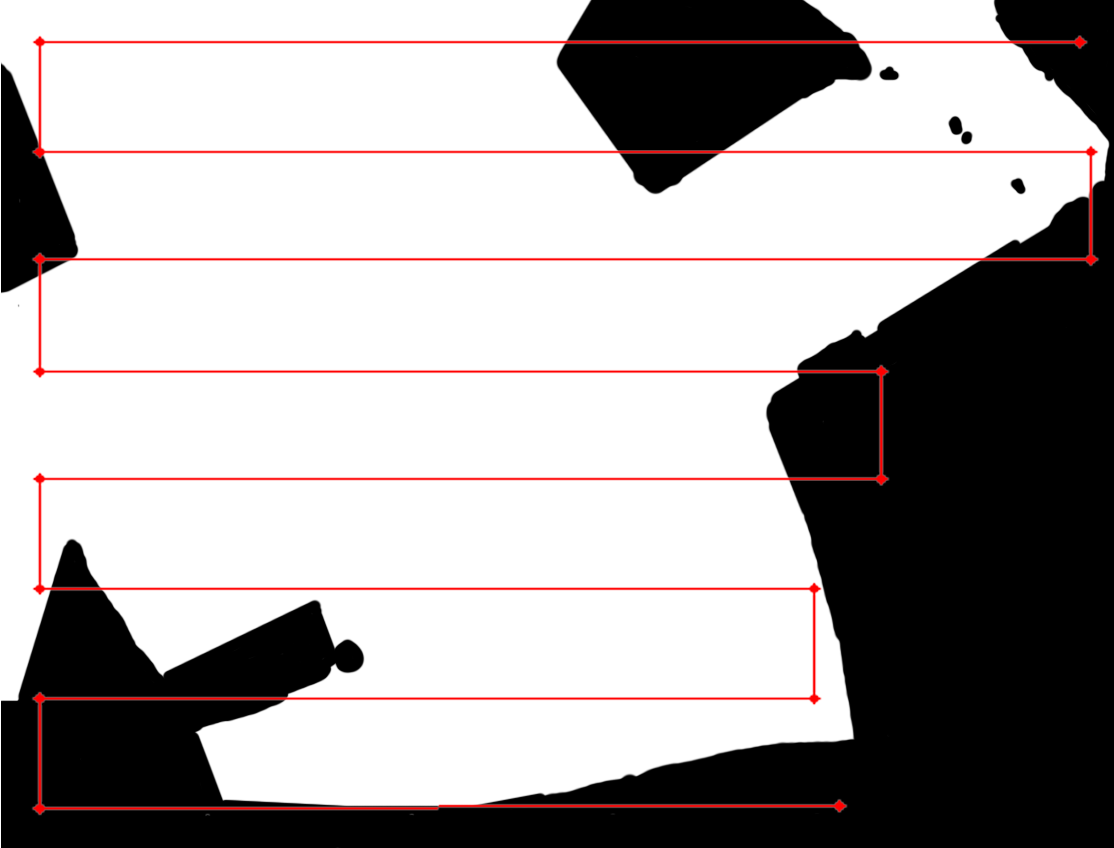
\includegraphics[width=0.49\textwidth]{calvisson2maskPath.png}}
%   \hfill
%   \subfigure[110 waypoints for 94.86\% of coverage]{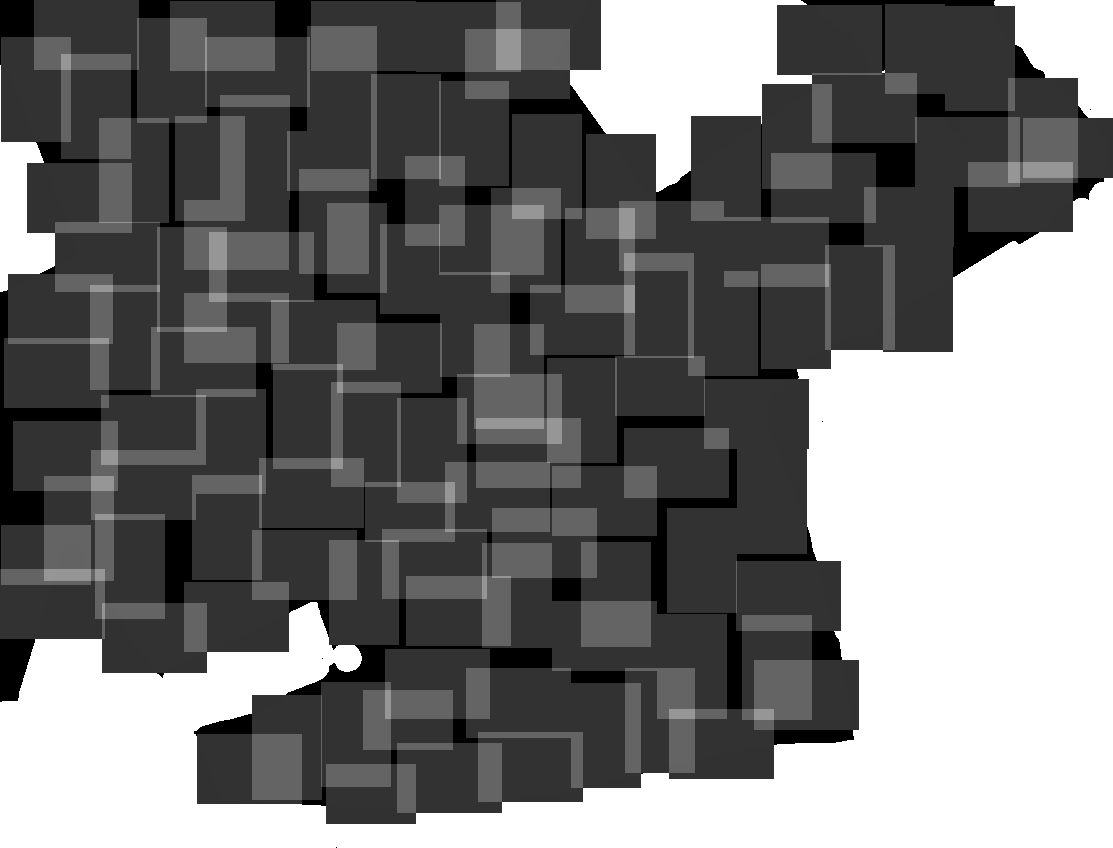
\includegraphics[width=0.49\textwidth]{zcalvisson2result1cout_94_862284_gen_3634_Ncam_110.png}}
%  
%  \subfigure[Path with 110 waypoints for 94.86\%  ]{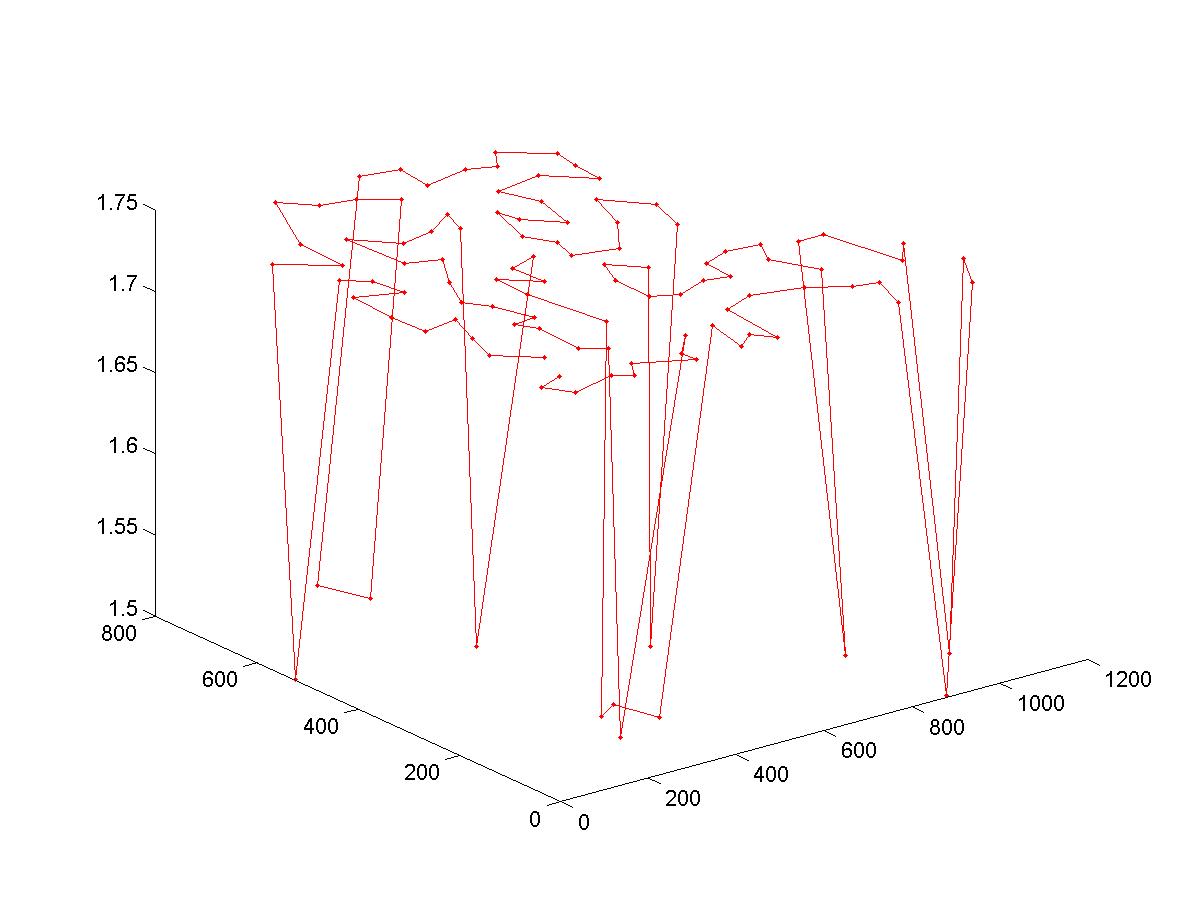
\includegraphics[width=0.85\textwidth]{zGAevolvTurnComplexCross_919Mut_001pop100cout_94_862284_gen_3634_Ncam_110Sorted.png}}
%  \caption{Room Coverage}\label{fig:trajectoryPath} 
%\end{figure}

 \begin{mfigures}[!]{optimisation of the path planing}{fig:trajectoryPath} \centering
\mfigure{width=.4\linewidth}{img/calvisson2maskPath.png}{Path planing using the pattern method.}{subfig:Dijktra}
\hspace{1cm}
\mfigure{width=.4\linewidth}{img/zcalvisson2result1cout_94_862284_gen_3634_Ncam_110.png}{Path compute with Dijktra multi goal.}{subfig:GATSP}
\mfigure{width=.4\linewidth}{img/zGAevolvTurnComplexCross_919Mut_001pop100cout_94_862284_gen_3634_Ncam_110Sorted.png}{Room Coverage.}{subfig:GATSP}
\end{mfigures} 
  In order to compare the efficiency of the trajectory computation proposed in this article with a standard method using a adapted pattern to cover an area. The patterned method apply is based on several article as \cite{63*,66*,pattern155*}
%  [ CHAO, Haiyang, BAUMANN, Marc, JENSEN, Austin, et al. Band-reconfigurable multi-UAV-based cooperative remote sensing for real-time water management and distributed irrigation control. In : IFAC World Congress, Seoul, Korea. 2008. \\]
%  [ ZHANG, Houxiang, ZHANG, Jianwei, et ZONG, Guanghua. Cleaning Trajectory Evaluation of a Wall Cleaning Robot Based on Synthesis Standards. In : Computational Engineering in Systems Applications, IMACS Multiconference on. IEEE, 2006. p. 1695-1700. \\]
%  [GALCERAN, Enric et CARRERAS, Marc. A survey on coverage path planning for robotics. Robotics and Autonomous Systems, 2013, vol. 61, no 12, p. 1258-1276.\\]. 
 %Predicate on the pattern method a path are compute on the area see fig ££££££££ calvison vide  £££££££££.
 The path proposed is establish on the area to cover and the camera field of view. The pattern is adapted depending then the shape of the area and the size of the camera projection in order to have a full coverage with the minimum of overlap. The final path using the pattern method as in figure \ref{fig:trajectoryPath}(a)
 \\In the other hand the solution proposed ( see figure \ref{fig:trajectoryPath}(b)) establish an path apparently more complex (see figure \ref{fig:trajectoryPath}(c)) using the third dimension with a coverage rate somewhat lower ( 94.86\% of coverage ).
 Although  the distance of the path  and the complexity trajectory based on  the equation \ref{Eq:trajectory} prove the efficiency of this method by a lower distance and a better complexity indicator as in table \ref{table:trajectory}.\\ 
 \begin{table}[t]
\begin{tabular}{|p{1.5cm}|p{1.8cm}|p{1.8cm}|p{1.8cm}|}
  \hline
   &Coverage rate & Path length (in px) &Trajectory complexity (eq:\ref{Eq:trajectory})  \\  \hline
  Pattern Method &  100\% & 9076 &90 \\ \hline
  Ours Method &  94.86\% & 8161 &69.81 \\ \hline
\end{tabular}
\caption{comparative table  of path distance and complexity.}\label{table:trajectory}
\end{table}
 
%  Dans cette partie on comapare des une methode  de calcule des trajectoire classique qui utilise des la repetition de paterne pour couvrire une zone.
%   l'avantage de la methode  utilisent des paternes et que l'on optien un taux de reconvrement beaucoup plus important qui  est de  100\% avec un taux de recouvremnt plus ou moin important. mais en contre partie l chemian parcourie et plus long, 200m contre 150m avec l'utilisation des algo génétique. concernant la complexité de la trajectoire  on s'appuit sur l'equation  

\subsection{Indore simulation} \label{experiment}

 \begin{mfigures}[!]{optimisation of the path planing}{fig:final_room2} \centering
%\mfigure{width=.4\linewidth}{img/room_python.PNG}{Poses of every image captured in the room}{subfig:RoomPy}
\mfigure{width=.4\linewidth}{img/room_full.png}{Room Coverage}{subfig:fullRoomPath}
\hspace{1cm}
\mfigure{width=.4\linewidth}{img/VrepMyOptimization.png}{Pose of every images with the path planning}{subfig:PathPlanning}
\mfigure{width=.4\linewidth}{img/VrepCellDecopo1.png}{Room in V-rep}{subfig:VrepCellsDecomp}

\tabsimuposeVrepPath
\end{mfigures} 

In order to experiment the proposed method for coverage path planning a simple indoor experiment is proposed to begin.
The experiment proposed is based on the one discussed previously on Section \ref{sec:expRectObstacle}.
To remind the experiment is made in a simulated room ($15 \times 14 m^2$). The area to cover is shown in the Figure \figref{subfig:fullRoomPath}. The camera parameter are the same $4 \times 3 m^2$ when $z$ is equal to one and the $z$ factor can be equal at [0.5;1,1;5] only for the waypoints positioning optimization. On the other hand the sweep is  computed with the camera at the maximum altitude to have the biggest area coverage possible.

Thanks to this first experiment the path planning appear as much more appropriate. The path planning obtained by our method propose a shorter path, 881.6 pixel long when  the path by sweep is  at 1137 pixel long.  The path  proposed by the sweep is longer notably by the return to this starting point but not only (the junction between the start and finish of the path is 245 pixel long, with mean the path usefull to fully cover the area is around 892 pixel long). Moreover the proposed path planning in addition  then the shorter path the trajectory complexity is also better (65.22$^\circ$ instead to 97.81$^\circ$ for the path with sweep).
Finally the proposed solution allow a better path planning thanks to this optimized waypoints despite the non complete coverage of the area. 



\subsection{coverage outdoor}\label{coverageOutDoor}

\subsubsection{Comparison of the trajectory.} \label{trajectoire path}
 
 \begin{mfigures}[!]{Experimentation of coverage path planning in the outside area.}{fig:FleyPathPlan} \centering
%\mfigure{width=.4\linewidth}{img/room_python.PNG}{Poses of every image captured in the room}{subfig:RoomPy}
\mfigure{width=.4\linewidth}{img/fig10-a2.png}{Path planing using the pattern method.}{subfig:FleytfullRoomPath}
\hspace{1cm}
\mfigure{width=.4\linewidth}{img/fig10-b2.png}{[80 waypoints for 98.28\% of coverage.}{subfig:FleyPathPlanning}
\mfigure{width=.4\linewidth}{img/fig10-c2.png}{Path with 80 waypoints for a distance of 4015.6 px.}{subfig:FleyCellsDecomp}

\tabsimuposeVrepPath
\end{mfigures} 
 
 
% \begin{figure}[t!]
%  \centering
%   \subfloat[Path planing using the pattern method.]{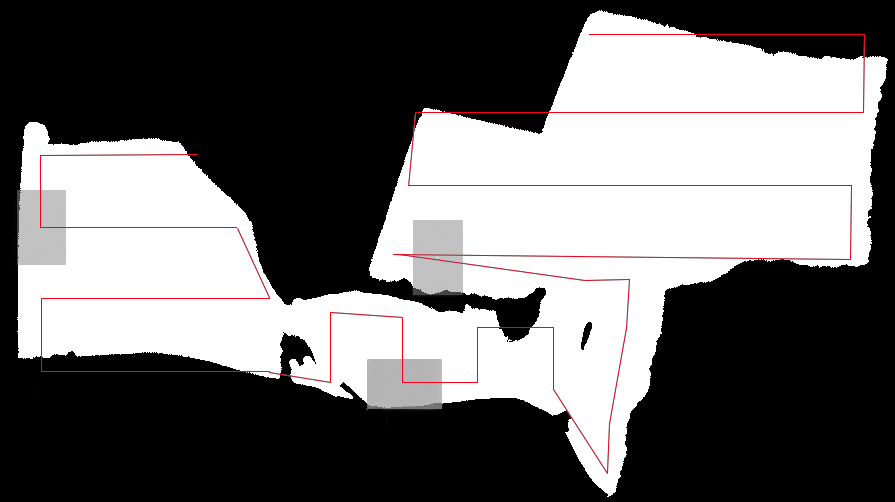
\includegraphics[width=0.475\textwidth]{fig10-a2.png}}\qquad
%   \subfloat[80 waypoints for 98.28\% of coverage.]{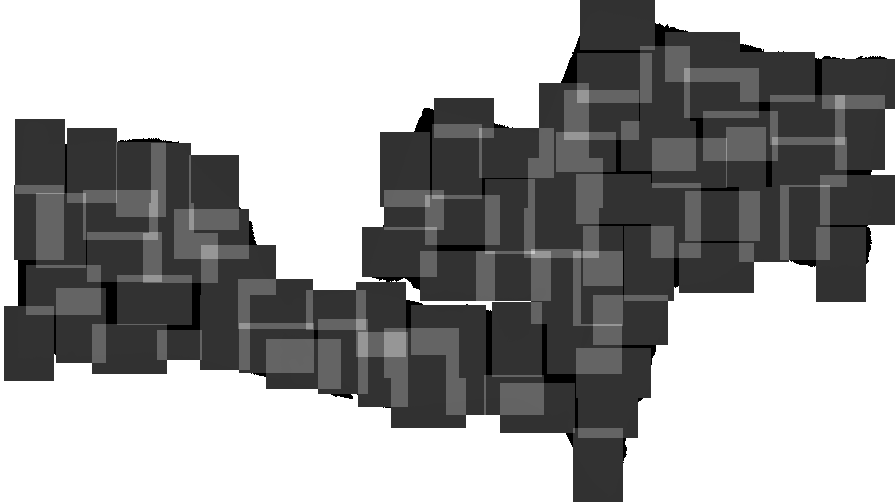
\includegraphics[width=0.475\textwidth]{fig10-b2.png}}\hfill %zcalvisson2result1cout_94_862284_gen_3634_Ncam_110
% %\subfloat[Path with 110 waypoints for 94.86\%  ]{\includegraphics[width=0.55\textwidth]{fig10-c.jpg}}%zGAevolvTurnComplexCross_919Mut_001pop100cout_94_862284_gen_3634_Ncam_110Sorted  width=0.45
% \hfill %zcalvisson2result1cout_94_862284_gen_3634_Ncam_110
% \subfloat[Path with 80 waypoints for a distance of 4015.6 px. ]{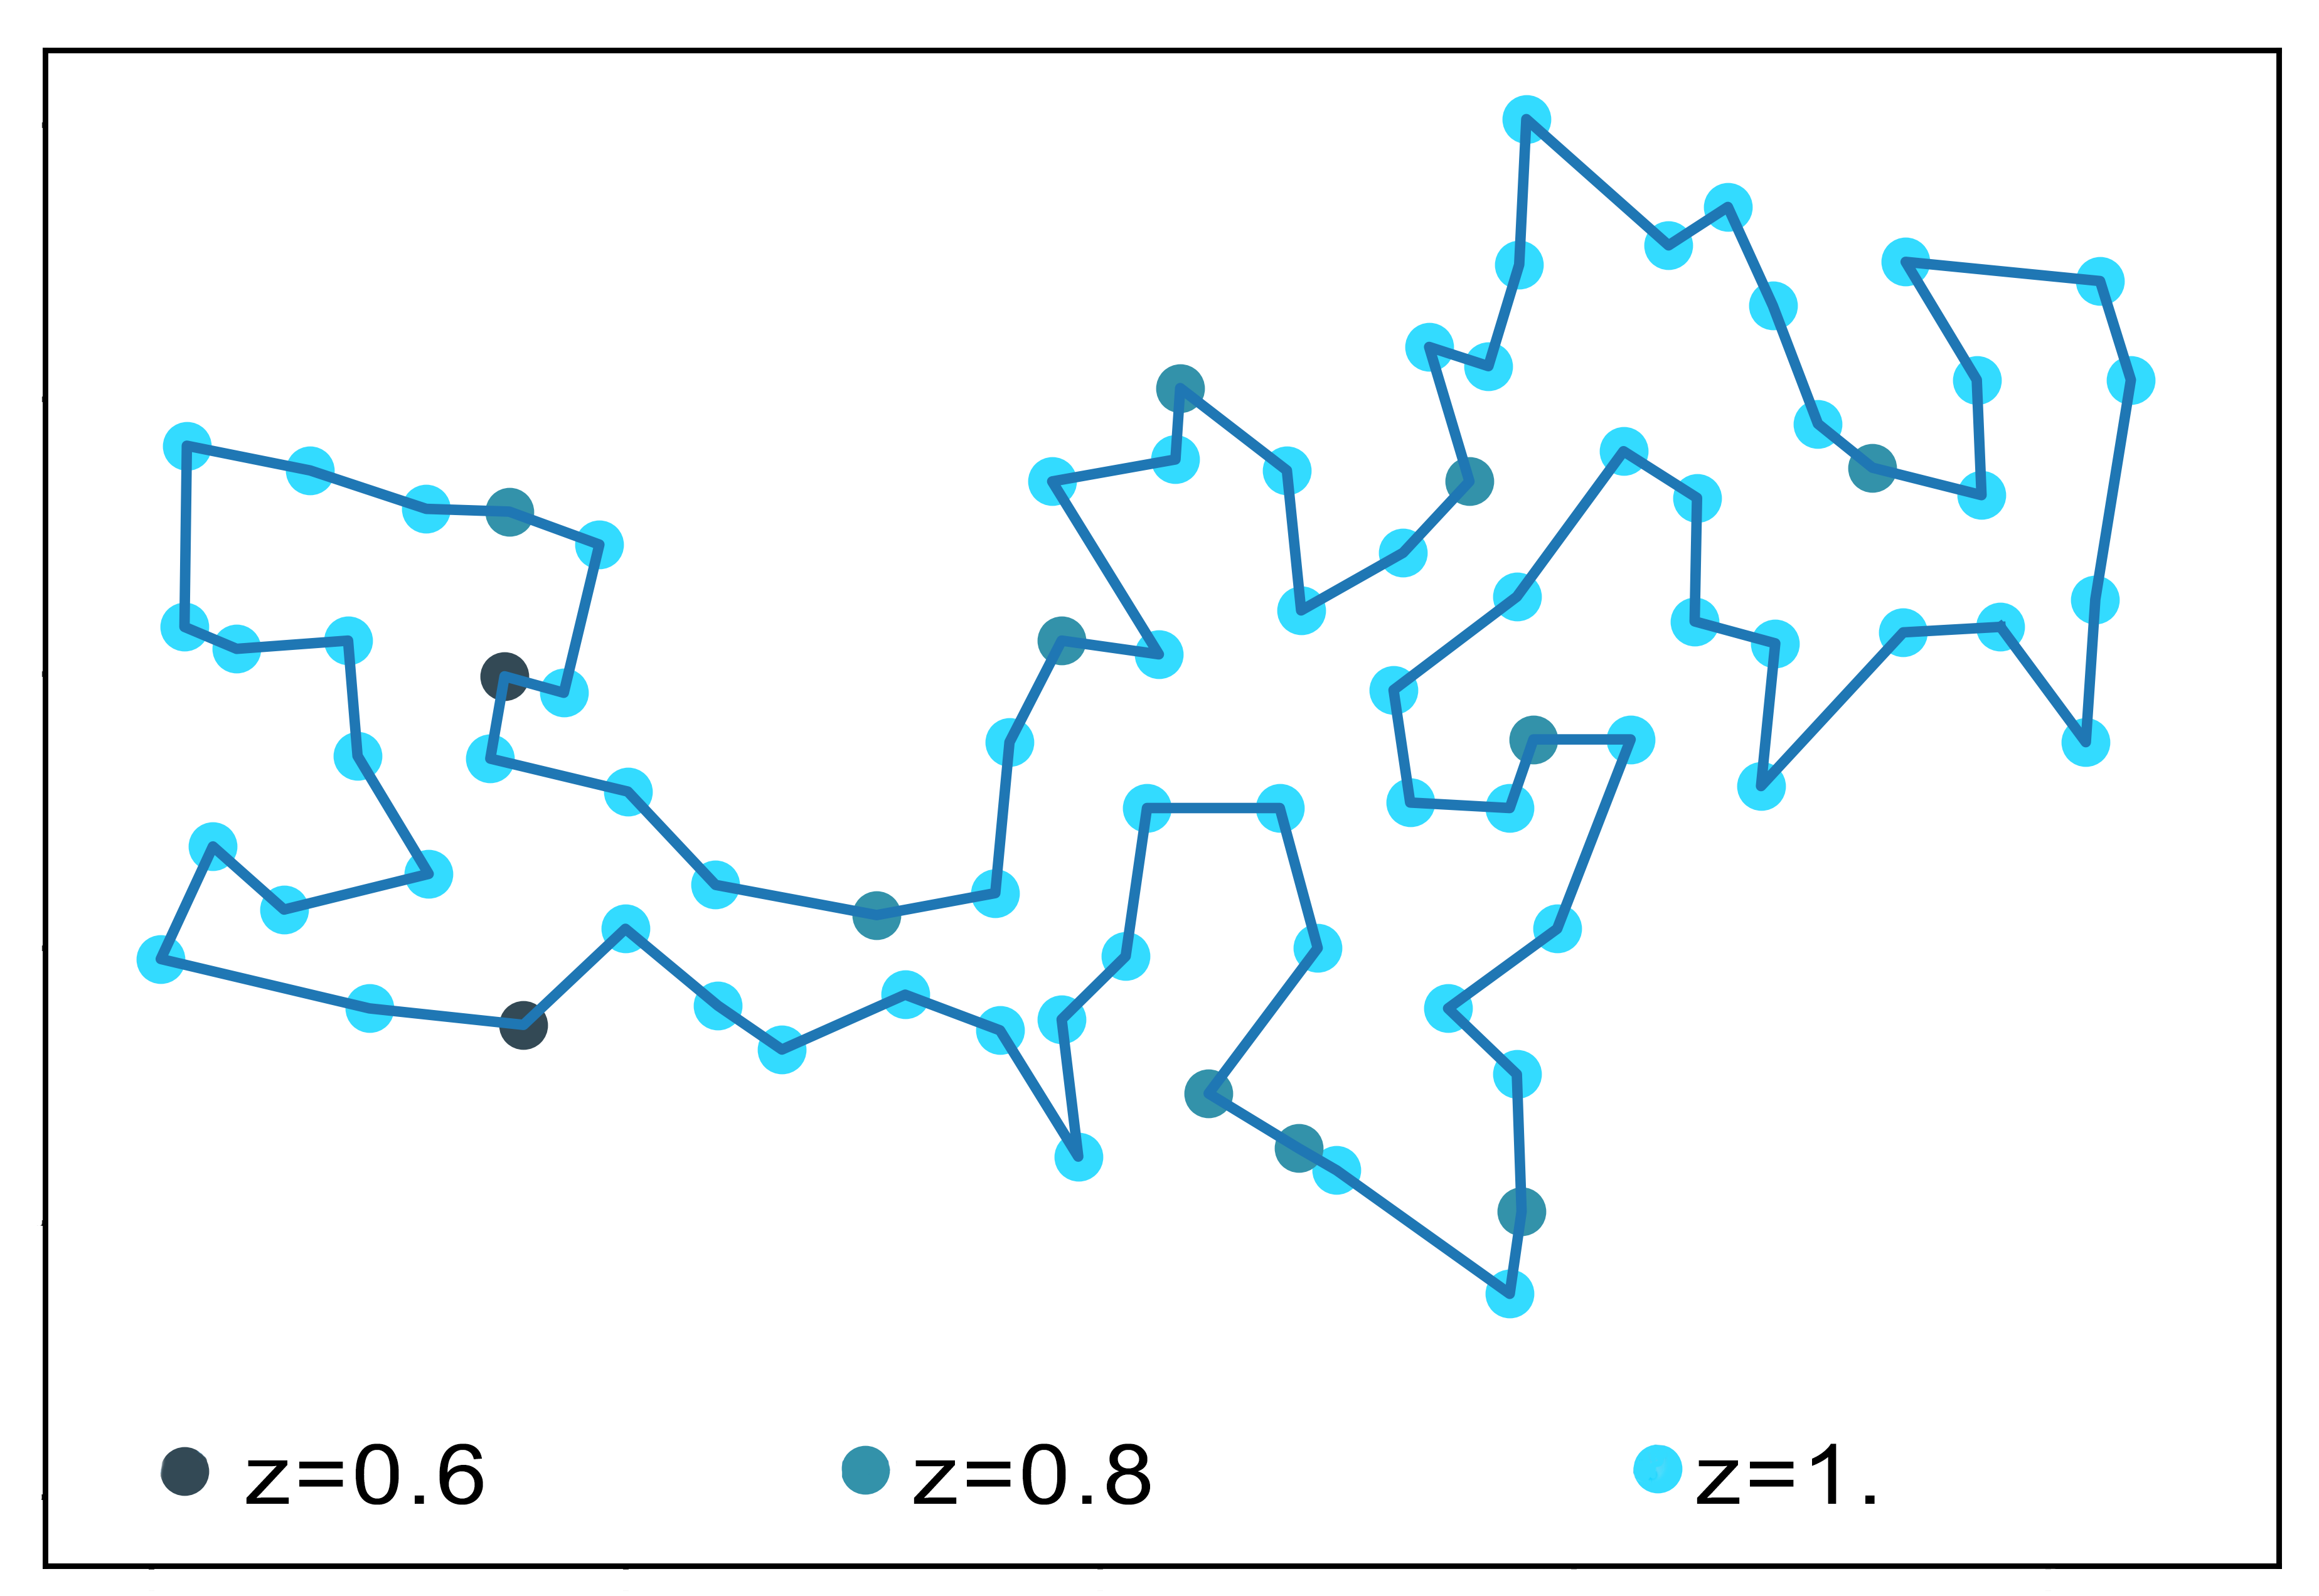
\includegraphics[width=0.45\textwidth]{fig10-c2.png}} \hfill
% \subfloat[][]{\tabsimupp}
%  %zcalvisson2result1cout_94_862284_gen_3634_Ncam_110
% %\subfloat[Path with 110 waypoints for 94.86\%  ]{\includegraphics[width=0.45\textwidth]{fig10-d_bis.jpg}}
%  \caption{Experimentation of coverage path planning in the outside area.}\label{fig:trajectoryPath} 
%\end{figure}

%\begin{table}[]
%\centering
%\caption{Outdoor simulation with path planing (Figure \ref{fig:trajectoryPath})}
%\label{pathPlan}
%\begin{tabular}{l|ll}
%\textbf {Parameters }             &\textbf{Value }                              &  \\ \cline{1-2}
%\cellcolor[HTML]{FFFFFF}{$z$}        & \cellcolor[HTML]{FFFFFF}{[}1;1,5;2{]}        &  \\
%\cellcolor[HTML]{F2F2F2}$\gamma$        & \cellcolor[HTML]{F2F2F2}portrait or landscape &  \\
%\cellcolor[HTML]{FFFFFF}Coverage & \cellcolor[HTML]{FFFFFF}waypoint snap        &  \\
%\cellcolor[HTML]{F2F2F2}Maximum size of camera projection & \cellcolor[HTML]{F2F2F2}70x105px             & 
%\end{tabular}
%\end{table}
%\begin{table}[]
%\centering
%\caption{Outdoor simulation with path planing(Figure \ref{fig:trajectoryPath})}
%\label{tab:pathPlan}
%\begin{tabular}{l|ll}
%\textbf {Parametres }             &\textbf{Value }                              &  \\ \cline{1-2}
%\cellcolor[HTML]{FFFFFF}{$z$}        & \cellcolor[HTML]{FFFFFF}{[}1;1,5;2{]}        &  \\
%\cellcolor[HTML]{F2F2F2}$\gamma$        & \cellcolor[HTML]{F2F2F2} portrait or landscape &  \\
%\cellcolor[HTML]{FFFFFF}Coverage & \cellcolor[HTML]{FFFFFF} stream record        &  \\
%\cellcolor[HTML]{F2F2F2}Maximum size of camera projection & \cellcolor[HTML]{F2F2F2}70x105px             & 
%\end{tabular}
%\end{table}

  To compare the efficiency of the trajectory computation proposed in this article with a standard method, in term of coverage, path plan distance and trajectory complexity. The standard method used for CPP uses an adapted pattern to cover an area. The patterned method application is based on several articles as \citep{144*torres2016,191*di2016,63*chao2008,66*galceran2013} 119* %pattern155*

 The path proposed is established in the area to cover and the camera FoV. The pattern is adapted depending on the shape of the area and the size of the camera projection in order to have full coverage with the minimum of overlapping. The final path using the pattern method showed in Figure \ref{fig:trajectoryPath}a.
 \\ The solution proposed ( Figure \ref{fig:trajectoryPath}b) establishes a path apparently more complex (see Figure \ref{fig:trajectoryPath}c) using the third dimension with a coverage rate somewhat lower, 98.28\% of coverage for the full area after 3101 generation.
 Although the distance of the path and the complexity trajectory based on  Eq.(\ref{Eq:trajectory}) prove the efficiency of this method by a shorter distance and a better complexity indicator as depicted in Table \ref{table:trajectory}.\\ 
 \begin{table}[t]
\begin{tabular}{|p{1.5cm}|p{1.8cm}|p{1.8cm}|p{1.8cm}|}
  \hline
   &Coverage rate & Path length (in px) & Trajectory complexity (Eq.\ref{Eq:trajectory})  \\  \hline
  Pattern Method &  100\% & 4362.66 &82.14 \\ \hline
  Ours Method &  98.28\% & 4015.6 &65.78 \\ \hline
\end{tabular}
\caption{Comparative table  of path distance and complexity.}\label{table:trajectory}
\end{table}





%\begin{figure}[t]
%  \centering
%  \hspace*{\fill}
%  \subfigure[]{\label{subfig:satimg+mask}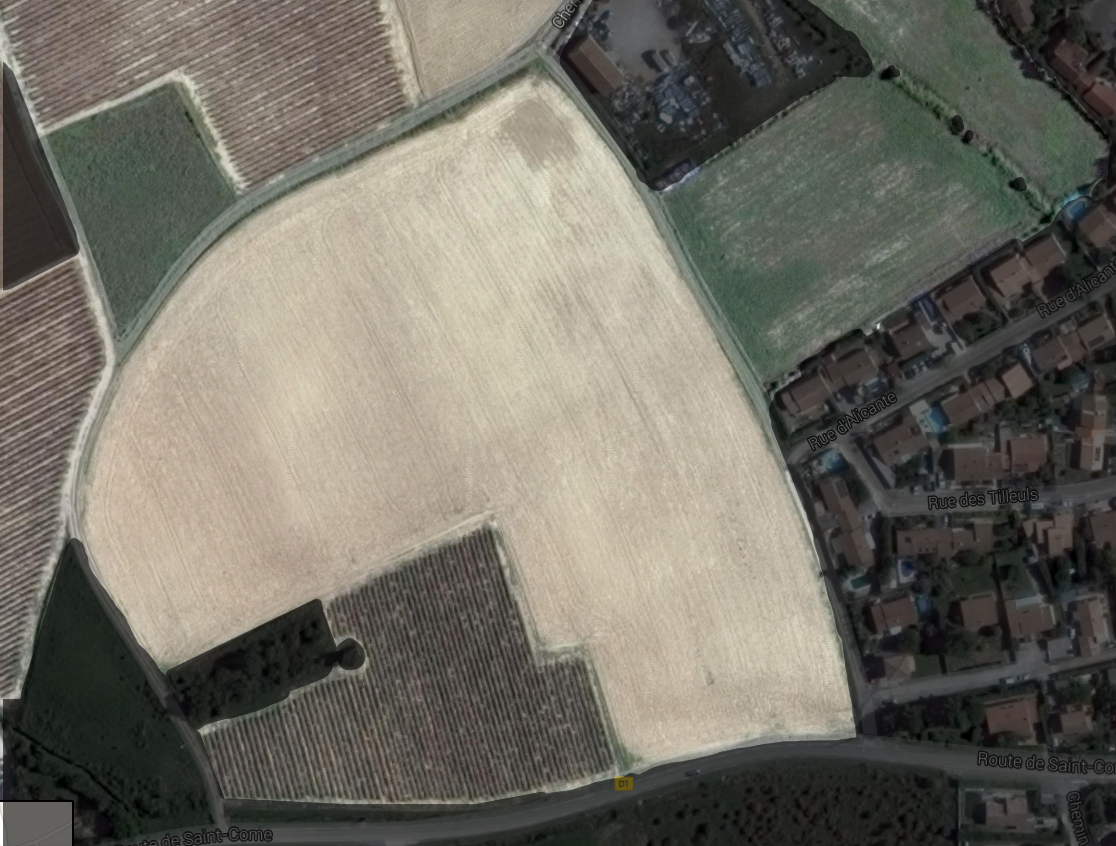
\includegraphics[width=0.48\linewidth]{calvisson2+mask.png}} \hfill
%  \subfigure[]{\label{subfig:satimgMask}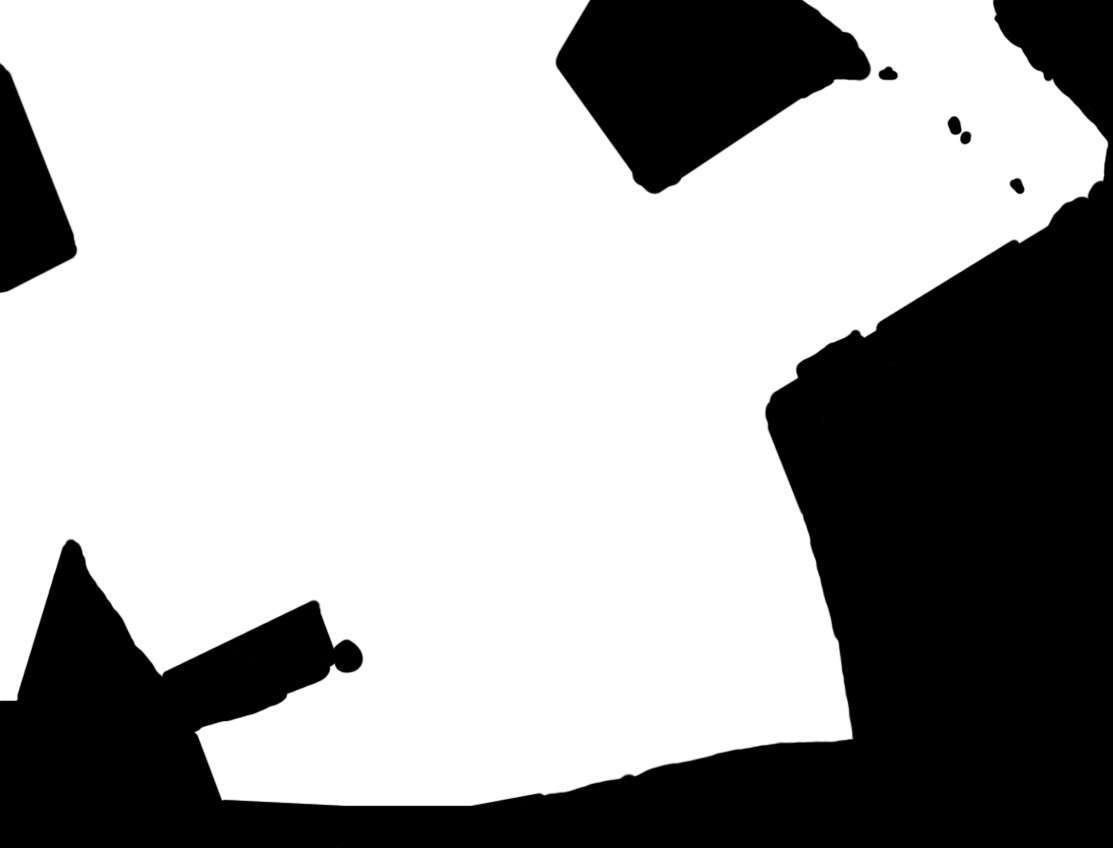
\includegraphics[width=0.49\linewidth]{calvisson2mask.png}}
%  \hspace*{\fill}
%  \\
%   \hspace*{\fill}
%  \subfigure[]{\label{subfig:satimgcoverage}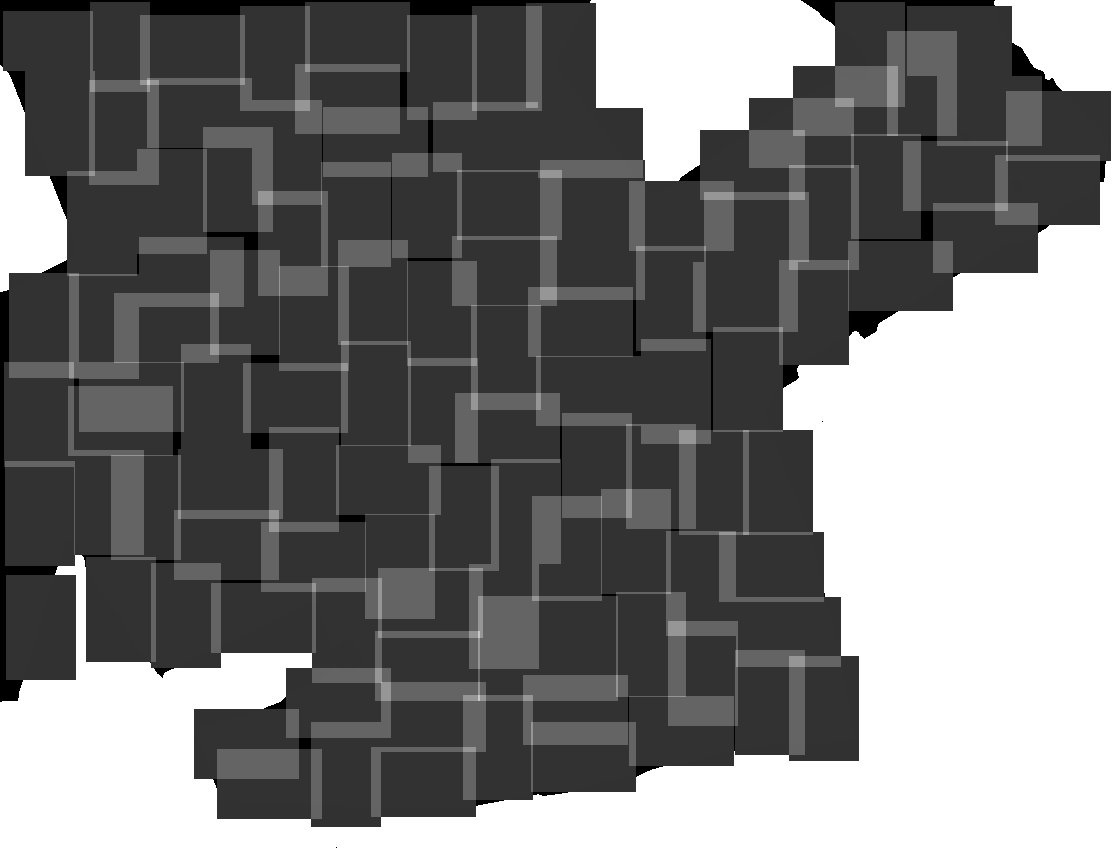
\includegraphics[width=0.80\linewidth]{zcalvisson2result1cout_98_260375_gen_170501_Ncam_110.png}}
%  \hspace*{\fill}
%  \hspace*{\fill}
%  \subfigure[]{\label{subfig:satimgNoncover}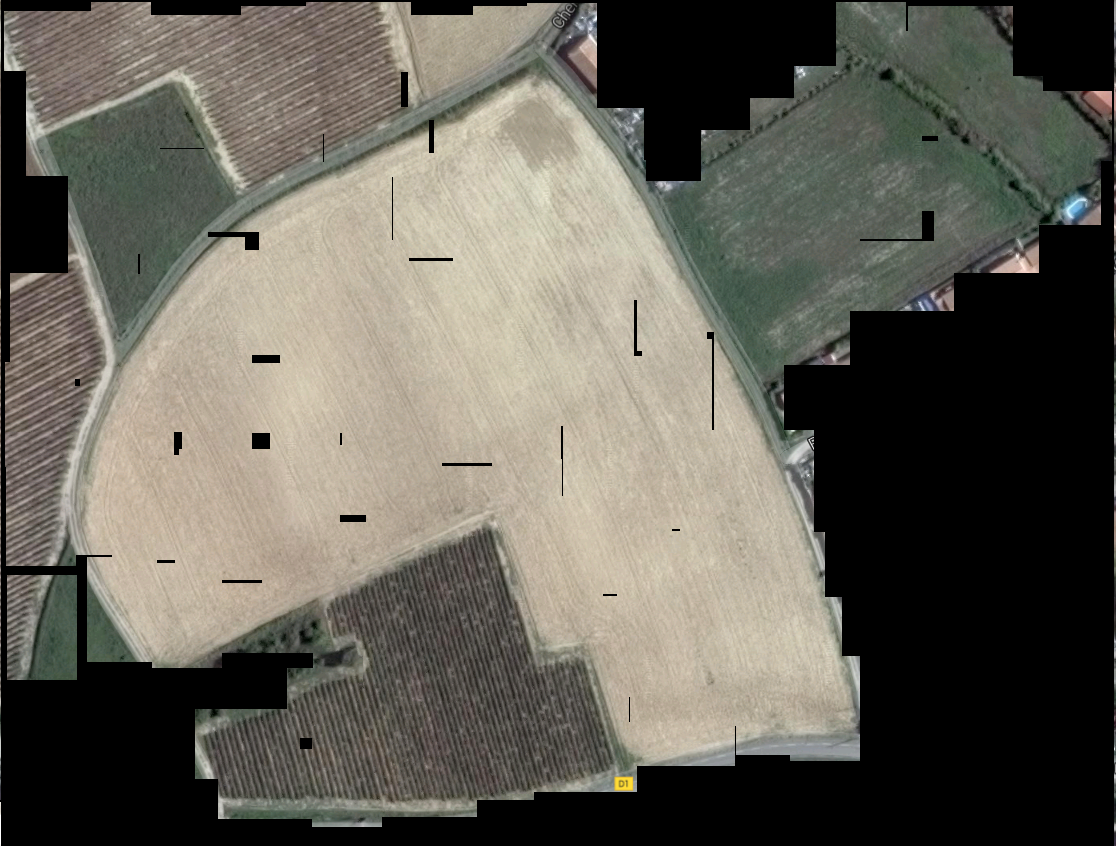
\includegraphics[width=.8\linewidth]{calvisson3cover.png}} \hfill
%  \hspace*{\fill}
%  \caption{ Optimization of the waypoint pose with a big outside area: (a) is the area to cover take form a satellite images,(b) is a mask of the area to cover, (c) is a result of the coverage with the waypoint position, (d) is the representation of the black hole.}
%  \label{fig:Rooms_shapes}
%\end{figure}
\subsubsection{Vast and complex outdoor}\label{sec:fey_map_CPPP}
\subsubsection{Biggest map with numerous waypoints}

\section{Use GA with non splitting in sub problem }
		\subsection{Explosion  de la complexité }
		\subsection{Result }
Use GA with non splitting in sub problem
			Explosion  de la complexité 
			Result 

%%%%%%%%%%%%%%%%%%%%%%%%%%%%%%%%%%%%%%%%%%%%%%%%%%%%



